\chapter{Introduction} \label{Introduction}
\minitoc

\section{Overview}

\subsection{DeFi pictures}

%%%% DeFi pictures
The use of technology in financial services is not new. Most transactions at banks or other financial services companies are accomplished with the help of technology nowadays. However, the role of technology is restricted to being a facilitator of such transactions. Companies still have to contend with navigating the legalese of jurisdictions, competing financial markets, and different standards to make a transaction possible. With its stack of common software protocols and public blockchains to build them on, DeFi places technology at the front and center of transactions in the financial services industry.

DeFi is a blockchain-based financial infrastructure that has recently gained a lot of attraction. The term generally refers to an open, permissionless, and highly interoperable protocol stack built on public smart contract platforms, such as the Ethereum blockchain (see Ethereum white paper, Buterin, 2013). It replicates existing financial services in a more open and transparent way. In particular, DeFi does not rely on intermediaries and centralized institutions. Instead, it is based on open protocols and decentralized applications (DApps). Agreements are enforced by code, transactions are executed in a secure and verifiable way, and legitimate state changes persist on a public blockchain. Thus, this architecture can create an immutable and highly interoperable financial system with unprecedented transparency, equal access rights, and little need for custodians, central clearing houses, or escrow services, as most of these roles can be assumed by "smart contracts."

Cryptocurrencies are the “money” of the DeFi ecosystem. A cryptocurrency is a digital or virtual currency that is secured by cryptography, which makes it nearly impossible to counterfeit or double-spend. Many cryptocurrencies are decentralized networks based on blockchain technology – a distributed ledger enforced by a disparate network of computers. A defining feature of cryptocurrencies is that they are generally not issued by any central authority, rendering them theoretically immune to government interference or manipulation. They hold the promise of making it easier to transfer funds directly between two parties, without the need for a trusted third party like a bank or credit card company. These transfers are instead secured by the use of public keys and private keys and different forms of incentive systems, like Proof of Work or Proof of Stake.

In modern cryptocurrency systems, a user's "wallet" or account address, has a public key, while the private key is known only to the owner and is used to sign transactions. Fund transfers are completed with minimal processing fees, allowing users to avoid the steep fees charged by banks and financial institutions for wire transfers.

%%%% Economic view
%% Centralize vs Decentralize
% (3 financial services: trading, lending/borrowing, investment)
% Intermediaries

% Orderbook vs AMM (CEX vs DEX)

%% Socioeconomic aspect

%%%% Technical view
%% A sample of DeFi
\begin{figure}[h]
  \centering
  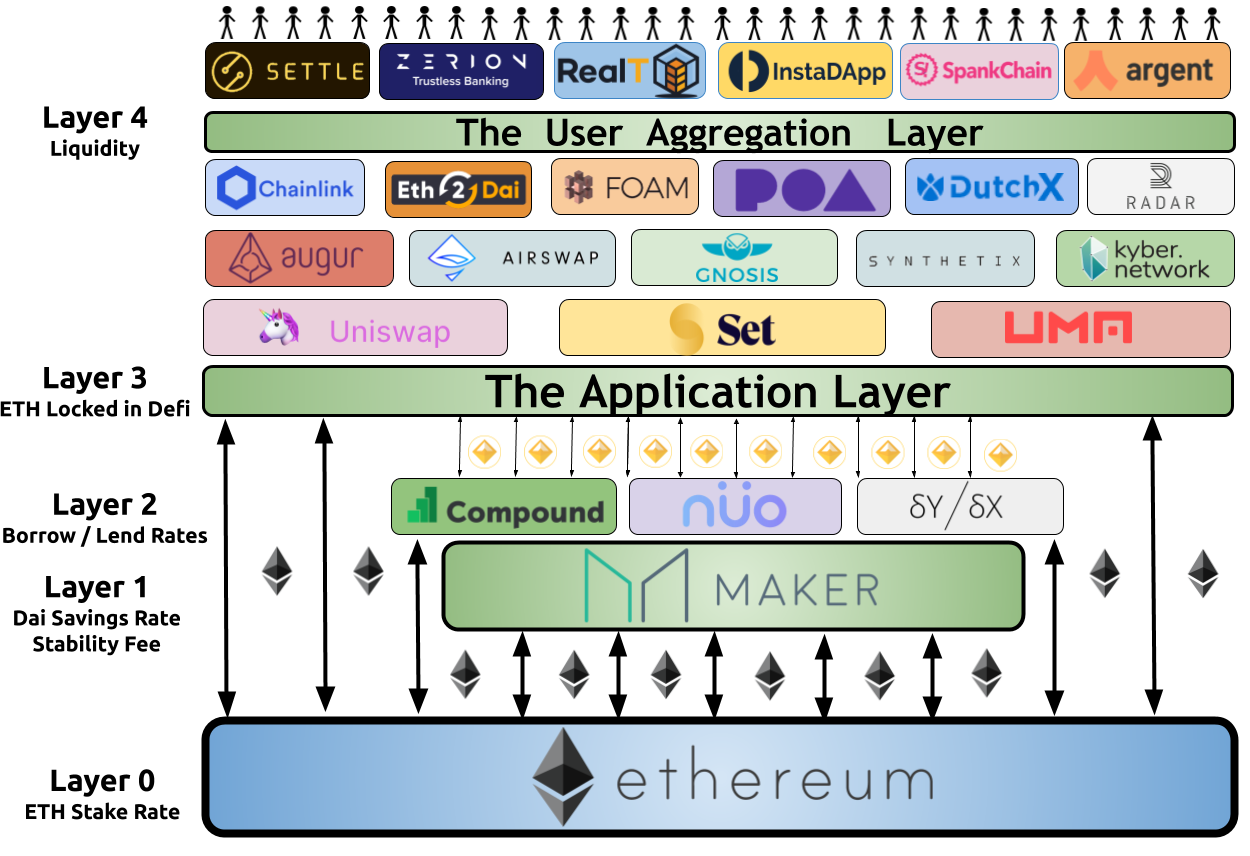
\includegraphics[width=.60\textwidth]{images/ethereum_building_blocks.png}
  \caption[Ethereum building blocks]{Ethereum building blocks}
  \label{fig:ethereum_building_blocks}
\end{figure}

Let take a look at the Ethereum building blocks (Ethereum digital finance layers) in \autoref{fig:ethereum_building_blocks}. As you can see, DeFi can carry out most of the necessary financial services: trade, lend and borrow, savings and spend. We can lend our asset on Compound and earn the interest rate, trade our Ethereum on Uniswap for other cryptocurrencies, and buy real estate on RealT. We can transfer money faster since there are no intermediaries and trusted third parties such as banks, ATMs,... Most of the financial services in the CeFi are digitalized in the DeFi systems.

%%%% DeFi ecosystem
% At first sight, blockchain is simply a distributed database and is not well known until late 2008. Bitcoin was 'born' by Satoshi Nakamoto to make an electronic payment system based on cryptography proof instead of trust. Satoshi makes use of digital signatures to improve the control of ownership, applies the PoW consensus to blockchain for preventing double-spending and securing the blockchain network. Then, with the help of smart contracts, Vitalik Buterin introduced Ethereum in 2013, a blockchain that are programmable. The Ethereum architecture can be simplify into five layers: aggregation layer, application layer, protocol layer, asset layer and settlement layer (\autoref{fig:defi_stacks}).

% \begin{figure}[ht!]
%   \centering
%   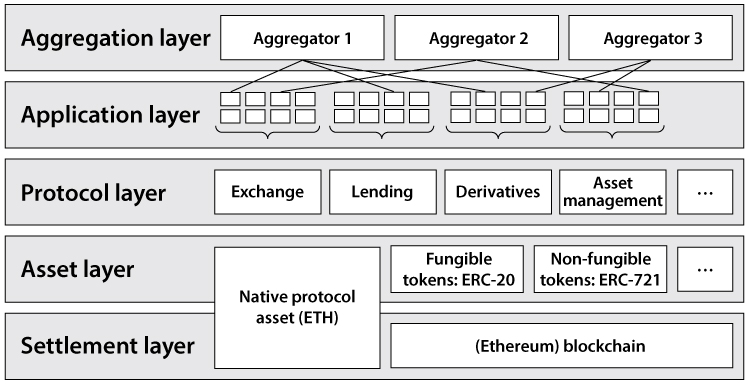
\includegraphics[width=.75\textwidth]{images/defi_stacks.jpg}
%   \caption[DeFi stacks]{DeFi stacks}
%   \label{fig:defi_stacks}
% \end{figure}

% From the bottom layer, blockchain is the core of the system, which acts as a database for any transaction. The native protocol asset is a mix of the asset layer and settlement layer, because the ETH is an incentive for mining block like Bitcoin. By mining a block, you contribute to the blockchain network: verify transactions and put them in a block, broadcast the block to the whole network, add it to the chain and confirm the added block then repeat. Protocol layer is where the protocol for financial services settled. DApps will implement these protocols to interact with the system. And on the aggregation layer, we can combine multiple DApps into a whole for end users, which will resemble a central bank internet application nowadays.


\subsection{Problem statements}


Now that we know about the financial structure of a DeFi system, let's analyze it as a software. The architecture of the DeFi system can be divided into two groups: on-chain and off-chain. On-chain means that they interact directly with the blockchain, includes the blockchain itself, DApps and the crypto wallets. Off-chain is the opposite of on-chain, they communicate with the blockchain through DApps or crypto wallet and has a GUI such as the web applications, mobile applications or desktop applications. The blockchain acts as a database for the system, and since its programmable using smart contracts, we call the application written in or connected to smart contracts on blockchain is DApps. The application is publicly viewed , either inside a block or open source, that's why it's decentralized and transparent. Crypto wallet helps the user manage they crypto assets and confirm transactions. A transaction flow is: first of all, the user creates and signs a transaction, then sends the transaction to the blockchain network for verifying the validity of the transaction and putting it into a block, which is performed automatically by DApps coded in smart contracts, finally the block contains the transaction is added to the chain and the transaction is succeeded. We can see DeFi is a kind of DApps providing financial services. By implementing the protocol for each individual service in smart contracts, DApps will behave accordingly on blockchain.

% What we are facing: CKD for the wallet
Crypto wallet is a crucial part of the system, as the users manage their assets through the use of the wallet. Rather than trusting the third parties or intermediaries, we prefer to cryptography since it's 'secure' and hard to break. The HD wallet uses asymmetric cryptography, whereas the user's address for receiving cryptocurrencies is the hash value of the public key, and the user's private key ensures that only the wallet's owner can sign and carry out a transaction. By any means, the cryptography algorithm used must be safe and cost-efficient. As recently RSA is broken and the Bitcoin had already applied elliptic curve cryptography (ECC), we will also work on ECC. Every transaction is needed to be signed by a different private key (we will explain why in our work) but stored all keys isn't efficient as there are thousands of transactions a day.

In order to keep the user's application lightweight, we need to find out a deterministic function to derive a hierarchical child key, or in short, a child key derivation (CKD) function. That's why we propose this idea as our thesis to improve the security of the wallet and reduce the hassle of key generation and management.

\section{Objectives}

% \subsection{Aims}

% CKD: Master public key -> child public key
Our aim is to create a CKD function for Ed25519, by which enhance the security and key management of a HD wallet. Another reason why we choose Ed25519 is that curve Secp256k1, used in bitcoin blockchain, is no longer a safe curve (\href{http://safecurves.cr.yp.to/disc.html}{SafeCurves}). Curve Ed25519 has some really good properties in terms of implementation security and speed of digital signatures (\href{https://cryptobook.nakov.com/digital-signatures/eddsa-and-ed25519}{CryptoBook}), as well as solid, well-tested libraries like NaCl for encryption and signatures. It's used in more and more elliptic curve crypto implementations these days and looks like it might become a standard for both digital signatures and public-key encryption. NIST (reference here) already has a draft for proposing updates to its standards on digital signatures and elliptic curve cryptography, adopting Ed25519.

\subsection{Practical benefits}

% Transaction speed: Sign and verify
By shifting to Ed25519, the wallet will be safer and the blockchain is also securer. As stated above, the security standards for ECC have been raised, proposed Ed25519 for digital signatures. Ed25519 is a fast and secure digital signature algorithm based on performance-optimized elliptic curves (curve Curve25519). Ed25519 is expected to quadruple performance versus Secp256k1 based on our preliminary benchmarking (\href{https://ripple.com/insights/curves-with-a-twist/}{Ripple}).

% Light-weight wallet
ECC can generate a subgroup with the same properties and doesn't reveal anything about its parent. In that way, ECC allows to safely generate a child key from the same master key, while if we keep using the same key in RSA it can be broken by the Chinese Remainder Theorem. Therefore; we only store the master key instead of storing a lot of keys for each account, reducing the size of the wallet.

% Secure and availability
% Better security and faster computing speed.

\section{Rationale of the study}

Our main focus is the blockchain technology and HD wallet on blockchain. This thesis will work on the breakthrough of the blockchain and how cryptography enhance the security of the blockchain network. For starter, blockchain solves the consensus problem (Byzantine General Problem \cite{DBLP:journals/toplas/LamportSP82}) of the distributed system, allow the network to tolerate the number malicious nodes up to nearly half of the nodes. With the help of asymmetric cryptography, blockchain further more improve the BFT to $n \geq f + 2$ (almost all of the nodes are malicious). Then we will focus on developing the HD wallet for Ed25519, specifically designing a CKD for Ed25519 and integrating it into the wallet.

\section{Tentative structure of the study}

is thesis contains 6 chapters. The contents are below:

\begin{enumerate}
  \item Introduce DeFi and its architecture
  \item Background knowledge about blockchain technology, HD wallet and cryptography
  \item The challenges we are facing and our approach to generate a CKD
  \item The goals that we want to achieve
  \item Some related works on improving the security of the system
  \item Conclusion and future work
\end{enumerate}

\section{Tentative schedule}

To make sure we understand DeFi from both technical view and financial view (in a certain amount), we divided our thesis into 5 main stages:

\textbf{Stage 1:} Study and research about the background of cryptography

\textbf{Stage 2:} Study and research about blockchain and blockchain wallet

\textbf{Stage 3:} Analyze the CKD of HD wallet on Secp256k1 and its approach

\textbf{Stage 4:} Propose a CKD for HD wallet on Ed25519

\textbf{Stage 5:} Implement the HD wallet on Ed25519

In the proposed thesis stage, we operate stage 1, 2, 3 of the thesis. In the thesis stage, we operate the remain stage.